\documentclass{article}

% if you need to pass options to natbib, use, e.g.:
% \PassOptionsToPackage{numbers, compress}{natbib}
% before loading nips_2017
%
% to avoid loading the natbib package, add option nonatbib:
% \usepackage[nonatbib]{nips_2017}

%\usepackage{nips_2017}

% to compile a camera-ready version, add the [final] option, e.g.:
\usepackage[final]{nips_2017}

\usepackage[utf8]{inputenc} % allow utf-8 input
\usepackage[T1]{fontenc}    % use 8-bit T1 fonts
\usepackage{hyperref}       % hyperlinks
\usepackage{url}            % simple URL typesetting
\usepackage{booktabs}       % professional-quality tables
\usepackage{amsfonts}       % blackboard math symbols
\usepackage{nicefrac}       % compact symbols for 1/2, etc.
\usepackage{microtype}      % microtypography

\usepackage{amsmath}	% for \begin{align}
\usepackage{graphicx}	% for \includegraphics{filename}
\usepackage{subcaption}	% for \begin{subfigure}[t]{0.5\textwidth}
\usepackage{enumitem}	% for using (a), (b), ...
\usepackage{courier}	% for \texttt{}

\newcommand{\bb}[1]{\boldsymbol{#1}}

\graphicspath{{fig/}}

\title{Progress Update}

% The \author macro works with any number of authors. There are two
% commands used to separate the names and addresses of multiple
% authors: \And and \AND.
%
% Using \And between authors leaves it to LaTeX to determine where to
% break the lines. Using \AND forces a line break at that point. So,
% if LaTeX puts 3 of 4 authors names on the first line, and the last
% on the second line, try using \AND instead of \And before the third
% author name.

\author{
	Yu-Hsiang Lin
		%\thanks{Use footnote for providing further information about author (webpage, alternative address)---\emph{not} for acknowledging funding agencies.}%
		\\
	Language Technologies Institute\\
	Carnegie Mellon University\\
	%\texttt{\{chianyuc, jeanl1, ziruil, yuhsianl, yuyanz1\}@andrew.cmu.edu} \\
	\texttt{yuhsianl@andrew.cmu.edu} \\
	%% examples of more authors
%	\And
%	Graham Neubig \\
%	Language Technologies Institute\\
%	Carnegie Mellon University\\
%	\texttt{gneubig@cs.cmu.edu} \\
  %% \AND
  %% Coauthor \\
  %% Affiliation \\
  %% Address \\
  %% \texttt{email} \\
  %% \And
  %% Coauthor \\
  %% Affiliation \\
  %% Address \\
  %% \texttt{email} \\
  %% \And
  %% Coauthor \\
  %% Affiliation \\
  %% Address \\
  %% \texttt{email} \\
}

\begin{document}
% \nipsfinalcopy is no longer used

\maketitle



% ---------------------------------------------------------
% ---------------------------------------------------------

\begin{abstract}

Place holder \cite{Adams2017}.

\end{abstract}

% ---------------------------------------------------------
% ---------------------------------------------------------

% ---------------------------------------------------------

\section{TTR using Language-independent tokenization}

Tokenizer: SentencePiece (https://github.com/google/sentencepiece)

Data: Spanish--English (/home/gneubig/exp/transfer-exp/data/spa\_eng)

For debugging purposes, we first consider English, and use only the training set (ted-train.mtok.eng) to train the tokenizer model. The number of sentences in this training set is 196,036.

Model: The model type is unigram, vocabulary size is 8,000, character coverage is 100\%.

If we run tokenizer on the same training dataset using this model, the TTR result is:

distinct token count = 7,989

token count = 5,386,583

TTR = 0.001483

Note that a few sample high-/low-frequency tokens are shown in Figures 1 and 2. Actually when it performs the tokenization, the UNK, BOS, EOS have been removed (Figure 3).

Should probably further remove things like ``quot'', ``\_\&'', and punctuations.

If I increase the vocabulary size to 16,000, the result is:

distinct token count = 15,981

token count = 5,232,195

TTR = 0.003054

Give more example of vocabularies in the middle in Figure 4.

(It seems that increasing vocabulary size of model will increase TTR, which indicates that the previous vocabulary size may be too small to be representative.)

vocabulary size = 32,000

distinct token count = 29,765

token count = 5,177,707

TTR = 0.005749

Vocabulary size larger than 32,000 seems to be too large. Encounter error during training: the training ends early and reports error

RuntimeError: Internal: /Users/travis/build/google/sentencepiece/src/trainer\_interface.cc(343) [(trainer\_spec\_.vocab\_size()) == (model\_proto->pieces\_size())]









\clearpage

\begin{figure}
\center
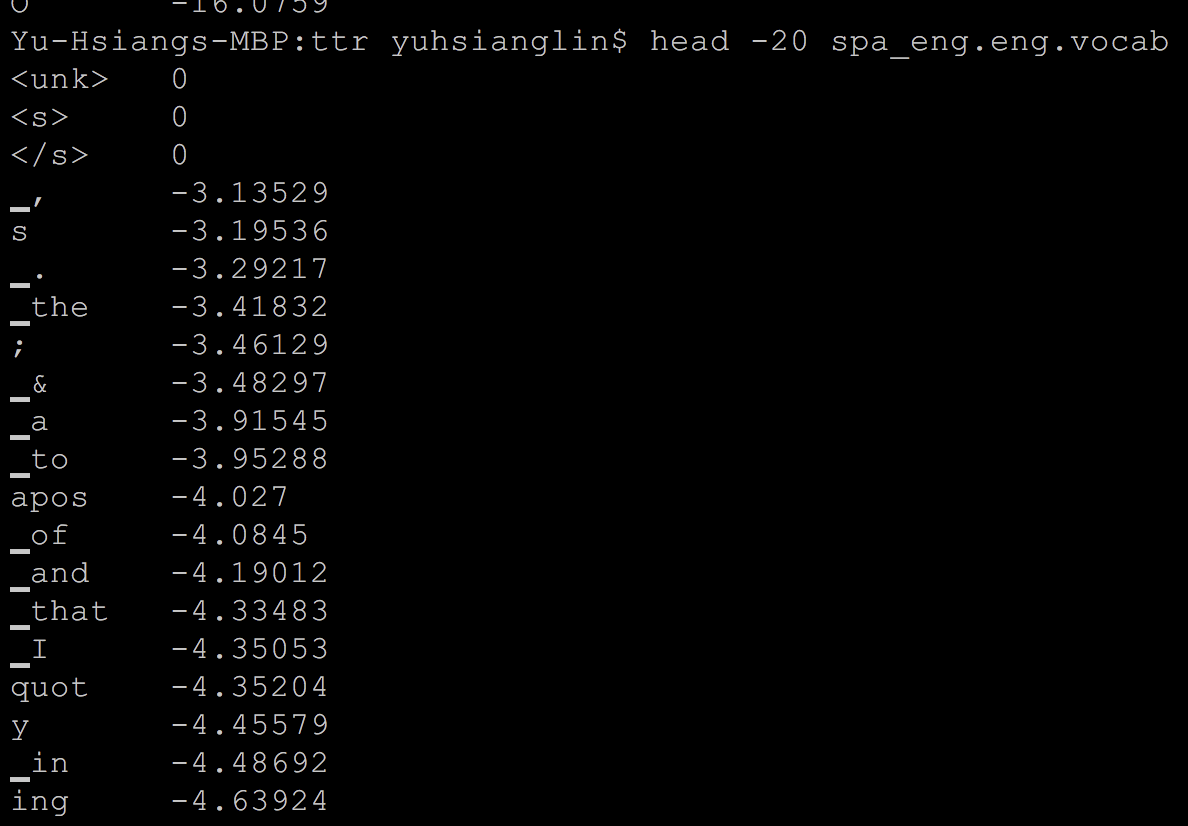
\includegraphics[width=12cm]{vocab1.png}\\
\caption{Top 20.}
\end{figure}

\begin{figure}
\center
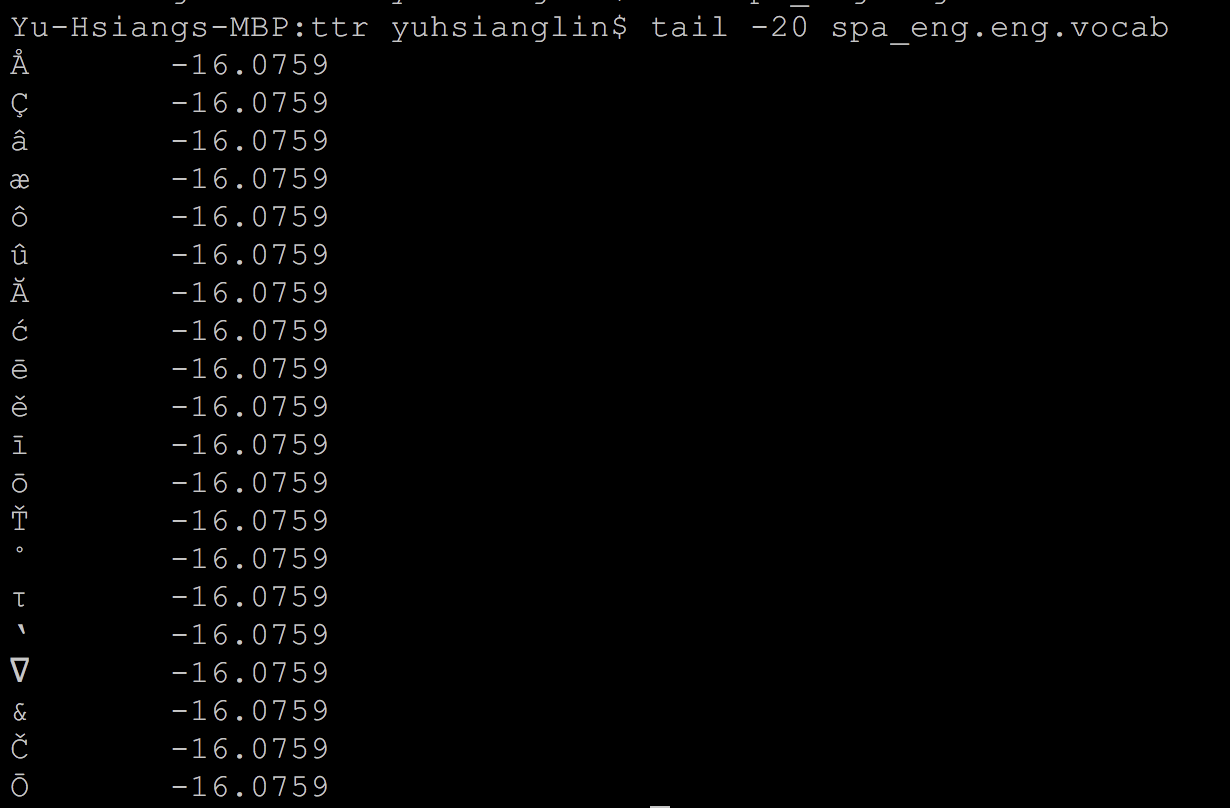
\includegraphics[width=12cm]{vocab2.png}\\
\caption{Tail 20.}
\end{figure}

\begin{figure}
\center
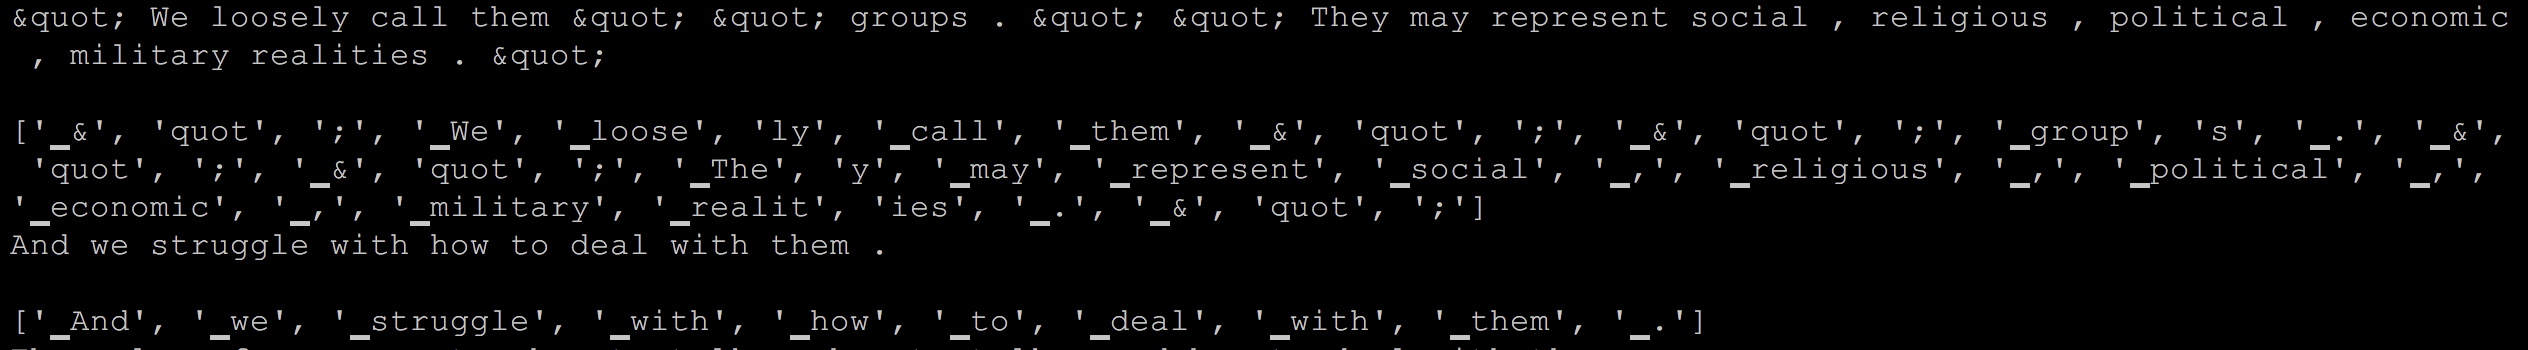
\includegraphics[width=16cm]{ex1.png}\\
\caption{Example.}
\end{figure}

\begin{figure}
\center
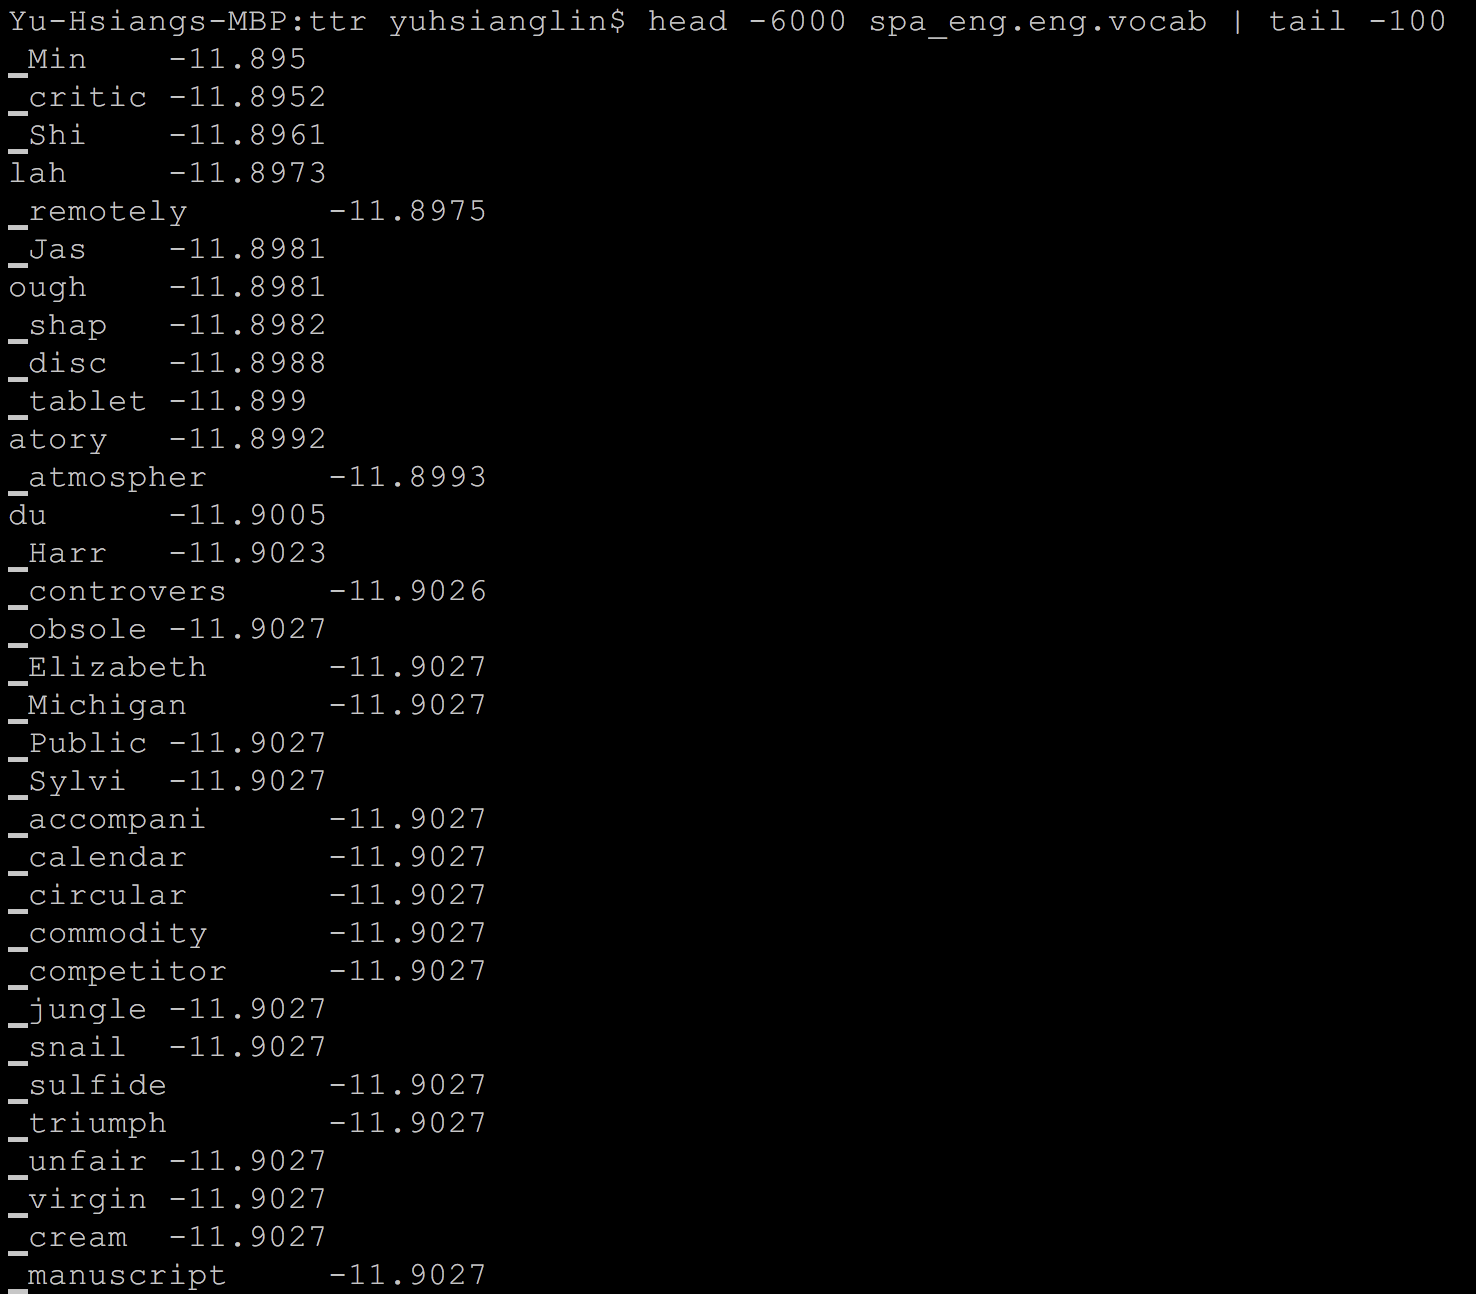
\includegraphics[width=12cm]{vocab3.png}\\
\caption{Middle (6000+).}
\end{figure}




% ---------------------------------------------------------
% ---------------------------------------------------------

%\subsubsection*{Acknowledgments}

% Use unnumbered third level headings for the acknowledgments.



% ----------------------------------------------------
% ----------------------------------------------------

\bibliographystyle{plain}
\bibliography{phonemebib}

\end{document}
